\documentclass[12pt]{article}

\usepackage[left=2.5cm,right=2cm,top=2cm,bottom=2cm]{geometry}
\setlength{\parindent}{0mm}

\usepackage{float}

\usepackage{parskip}
\usepackage[document]{ragged2e}
\usepackage[spanish]{babel}
\decimalpoint
\usepackage[utf8]{inputenc}
\usepackage{amsmath,amsthm,mathtools}
\usepackage{amsfonts,amssymb,latexsym}
\usepackage{enumerate}
\usepackage[dvips,usenames]{color}
\definecolor{RojoAnayelRey}{rgb}{1,.25,.25}
\usepackage{tikz}
\usepackage[bookmarks=true,
            bookmarksnumbered=false, % true means bookmarks in 
                                     % left window are numbered                         
            bookmarksopen=false,     % true means only level 1
                                     % are displayed.
            colorlinks=true,
            urlcolor=cyan,
            linkcolor=blue]{hyperref}
            
\usepackage{beton}
\usepackage[T1]{fontenc}

\newcommand{\cov}{\operatorname{cov}}

\title{ACP: Tareas varias finales de entrega voluntaria}

\author{David Cabezas Berrido}

\date{}

\begin{document}
\maketitle

\section{Código para limpiar los outliers}

Los valores que consideramos outliers son los que quedan fuera del
intervalo $[Q_1-1.5 IQR,Q_3+1.5 IQR]$, donde $Q_1$ y $Q_3$ son los
cuartiles 1 y 3, y $IQR=Q_3-Q_1$ es el rango intercuartil. En la
documentación de la función
\href{https://www.rdocumentation.org/packages/graphics/versions/3.6.2/topics/boxplot}{\texttt{boxpolt}}
podemos corroborar (parámtero \texttt{range=1.5} que R
también implementa este criterio, como era de esperar.

El motivo por el que hemos tenido que ejecutar el código para
modificar los outliers por el valor de la media es el siguiente:

Si sustituimos los valores de los outliers por la media de la columna,
la distribución se concentra más entorno a la media. Esto provoca que
los cuartiles se acerque más a la media y se reduca el rango
intercuartil. Por tanto, el intervalo $[Q_1-1.5 IQR,Q_3+1.5 IQR]$ se
hace más estrecho, y algunos valores que antes no considerábamos
outliers, ahora quedan fuera del intervalo.

Primero debemos plantearnos si estos son realmente outliers, ya que en
un principio los considerábamos valores ``no raros'' de la
distribución. Si nuestro único objetivo es conseguir una distribución
en la que todos los valores esten comprendidos en el intervalo antes
mencionado, entonces sí que deberíamos eliminarlos. En este caso, una
mejora simple a ejecutar el código varias veces sería automatizar el
proceso.

\begin{verbatim}
outlier<-function(data,na.rm=T){
  continue<-TRUE
  while(continue){
    H<-1.5*IQR(data)
    data[data<quantile(data,0.25,na.rm = T)-H]<-NA
    data[data>quantile(data,0.75, na.rm = T)+H]<-NA
    continue<-any(is.na(data))
    data[is.na(data)]<-mean(data,na.rm=T)
  }
  data
}
\end{verbatim}

Esta función sustituye los outliers por la media, y vuelve a realizar
este proceso mientras queden datos fuera del intervalo. Cuando toda la
distribución está comprendida en el intervalo correspondiente, de modo
que realiza las iteraciones justas y necesarias para cada columna.

Con una sola pasada de esta función (por cada columna) sobre el
ejemplo de \textit{Datos\_mundiales} conseguimos las distribuciones siguientes:

\begin{figure}[H]
  \centering
  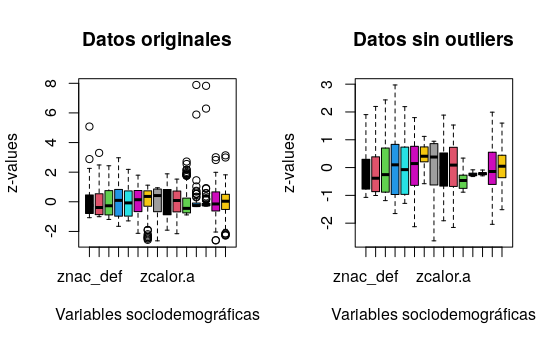
\includegraphics[width=140mm]{imgs/mundiales-outliers}
  \caption{Distribución de las variables antes y después de limpiar los outliers.}
\end{figure}

Observamos que hemos eliminado todos los outliers como
queríamos. Aunque se considere una ``mala práctica'' el uso de bucles
en R, no hemos utilizado un bucle para iterar sobre los datos, por lo
que el soporte para operaciones vectorizadas de R no podía ayudarnos
en esta tarea.

\section{Plot PCA en 3D}

Seguimos las indicaciones de
\href{https://cran.r-project.org/web/packages/pca3d/vignettes/pca3d.pdf}{https://cran.r-project.org/web/packages/pca3d/vignettes/pca3d.pdf}
para mostrar las variables en un cubo tridimensional con las tres
primeras componentes principales como ejes (Figura
\ref{fig:pca3d-instancias}). \textbf{El número que aparece junto a
  cada instancia es el número de instancia (hay 109), tanto en esta
  representación en 3D como en el 'Biplot' que vimos en la sesión.}

Usamos
\begin{verbatim}
pca3d(PCA,fancy=FALSE, show.shadows = FALSE, show.labels=TRUE)
\end{verbatim}

y obtenemos la siguiente representación:
\begin{figure}[H]
  \centering
  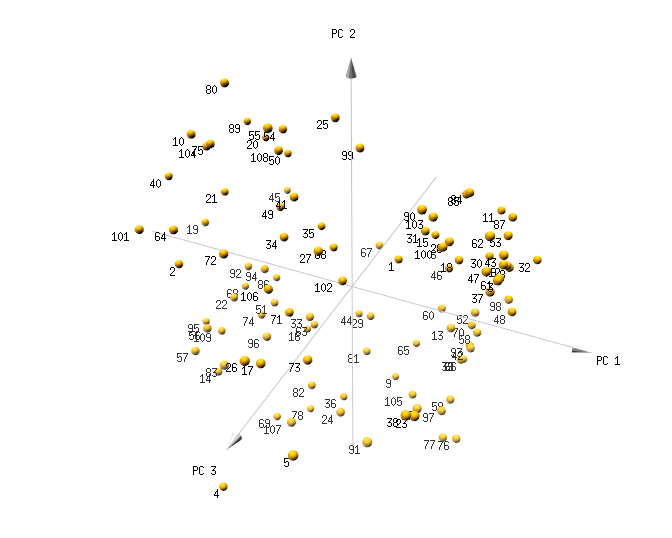
\includegraphics[width=100mm]{imgs/pca3d-instancias}
  \caption{Distribución de las instancias respecto a las tres primeras
    componentes principales.}
  \label{fig:pca3d-instancias}
\end{figure}

No he conseguido visualizar la contribución de cada variable a cada
componente principal cómodamente. Mi intento más cercano al éxito ha
sido una modificación de un
\href{https://stackoverflow.com/questions/44393823/3d-biplot-in-plotly-r}{código
  de \texttt{Stack Overflow}} que me ha pasado un compañero. He
obtenido lo siguiente:
\begin{figure}[H]
  \centering
  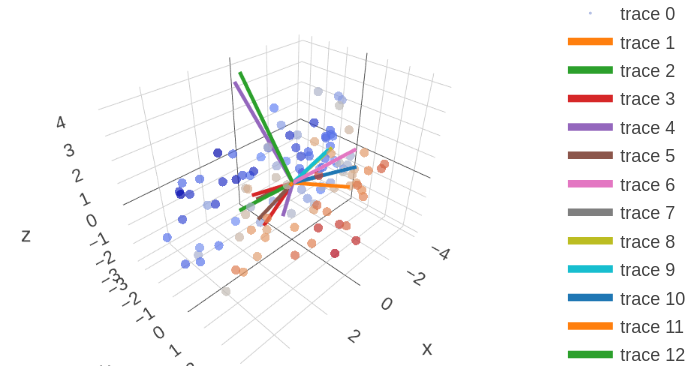
\includegraphics[width=100mm]{imgs/pca3d-variables}
  \caption{Contribución de las variables a cada una de las tres componentes principales.}
\end{figure}

En la leyenda obtenía las 15 variables bajando la barra, pero no se
reconoce a que variable representa cada línea. Una solución podría ser
ponerle un label dentro del gráfico en la punta de cada línea con el
nombre de la variable que representa. En su defecto, podría cambiar
los nombres de la leyenda por los nombres de las variables en lugar de
\texttt{trace X} (ahora mismo hay que contar el número de la variable
para saber de cual se trata) y utilizar una paleta de colores más
amplia para evitar que se repitiesen. No obstante, en Rstudio se puede pasar
el ratón por las líneas y ver a que número (no nombre) de variable
corresponden. He intentado ambas soluciones y he tenido algunos
problemas que no conseguí solucionar, decidí dejarlo así porque me
estaba llevando demasiado tiempo.

\section{Interpretación de las coordenadas en la base formada por las componentes principales}

La línea a la que se refiere el enunciado (\texttt{PCA\$x}) no encaja
con la descripción que proporciona luego (\texttt{PCA\$rotation}),
pero con ambas obtenemos una matriz con coordenadas en la base formada
por las componentes principales. Interpretaremos ambas
coordenadas. Llamaremos $B$ a la base de $\mathbb{R}^{11}$ (se miden
las concentraciones de 11 elementos químicos) formada por las
variables de las que disponemos, las concentraciones de cada uno de
los elementos. Debido a la naturaliza de las variables, la totalidad
de la distribución estará en el cono positivo ${\mathbb{R}^+_0}^{11}$.
Con $B_{PCA}$ nos referiremos a la base de $\mathbb{R}^{11}$ formada
por las componentes principales.

Utilizando \texttt{PCA\$x}, obtenemos una matriz que en cada fila
contiene las coordenadas de una instancia del conjunto de datos (una
muestra de vídreo), en la base $B_{PCA}$. Al tomar las tres primeras
componentes principales, nos estamos quedando con la proyección sobre
un subespacio vectorial de tres dimensiones. Con el Análisis de
Componentes Principales se consigue una base de forma que el conjunto
de datos esté contenido en la mayor medida posible en hiperplanos de
menor dimensión, para así perder la menor información posible al
realizar la proyección.

Utilizando \texttt{PCA\$rotation}, obtenemos la matriz de cambio de
base entre $B$ y $B_{PCA}$. En la columna $i$-ésima están las
coordenadas del $i$-ésimo vector de $B_{PCA}$ (la $i$-ésima componente
principal) expresadas en la base $B$. Utilizando el convenio de
multiplicar con la matriz a la izquierda y el vector columna a la
derecha, esta sería la matriz de cambio de base de $B_{PCA}$ a
$B$. Como se trata de dos bases ortonormales, la matriz que realiza el
cambio inverso es su transpuesta, de modo que en la fila $i$-ésima
tenemos las coordenadas del $i$-ésimo vector de $B$ (el $i$-ésimo
elemento químico) expresadas en la base $B_{PCA}$.

La aplicación proyección sobre el espacio de tres dimensiones formado
por las tres primeras componentes principales tiene en la base
$B_{PCA}$ una expresión matricial con una matriz $3\times 11$ con tres
unos en la diagonal principal y el resto ceros. Multiplicando esa
matriz a la izquierda por la matriz transpuesta (a la derecha) de la
matriz de rotación (lo que equivale a quedarnos con las 3 primeras
filas, las correspondientes a las tres primeras componentes
pricipales), obtenemos una matriz (composición) que lleva una
instancia con coordenadas en $B$ a su proyección sobre el espacio
formado por las tres primeras componentes principales.

En el caso del sodio (Na), sus coordenadas en la $B$ son
$(0,0,0,0,1,0,0,0,0,0,0)^T$, y sus coordenadas en las tres primeras
componentes principales son $(0.35856892,0.10078347,-0.21389143)$ esto
significa que si una muestra de vídreo tiene una alta concentración de
sodio y una baja concentración del resto de materiales, sus
coordenadas en el nuevo espacio 3-dimensional estarán cerca de ser
proporcionales a $(0.35856892,0.10078347,-0.21389143)$, según las
concentraciones del resto de materiales.
\end{document}
